\documentclass[12pt,a4paper]{article}

\usepackage{geometry}
 \geometry{
 a4paper,
 total={170mm,257mm},
 left=20mm,
 top=20mm,
 }
 
\usepackage[english]{babel}
\usepackage[utf8]{inputenc}
\usepackage{amsmath}
\usepackage{amsfonts}
\usepackage{bm}
\usepackage{graphicx,caption,subcaption,float}

\bibliographystyle{ieeetr}

\title{APC524 Final project report
\\Time series analysis in python}

\author{Wenyan Gong, Zongxi Li, Cong Ma
\\Qingcan Wang, Zhuoran Yang, Hao Zhang
\\Princeton University}

\date{\today}

\begin{document}
\maketitle

\section{Project objective}
Time series analysis comprises methods for analyzing time series data in order to extract meaningful statistics and other characteristics of the data. It’s widely used in statistics, signal processing, pattern recognition, mathematical finance, weather forecasting, earthquake prediction, control engineering, and largely in any domain of applied science and engineering which involves temporal measurements. 

In this project, we will play a game with time series in finance. It has gained its popularity in Wall Street recently, since it is fundamental to the most promising quantitative investment strategies. We develop a system that can predict future prices of stocks, with different time series models. 

\begin{figure}[H]
        \centering
     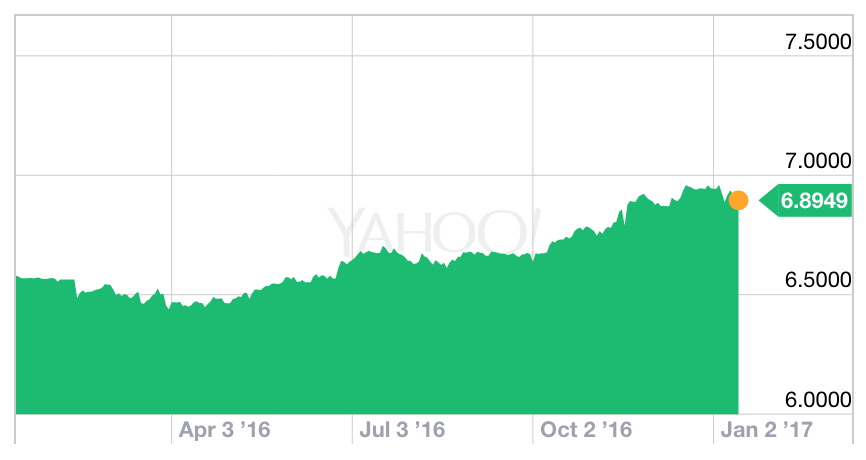
\includegraphics[width=.5\linewidth]{./Figure/USD-CNY.png}
\caption{USD to CNY exchange rate. Jan 12 2016 - Jan 12 2017. Source, Yahoo finance.}
\end{figure}

Given input of a stock price series, our system will first fit some powerful and popular time series models, such as autoregressive (AR) model, moving average (MA) model and other derived models. This procedure will give you the estimation of parameters in these models. 

The most important task in estimation is the optimization procedure. Users can select one of optimization methods in the system based on their preference. The optimization method includes but not limited to gradient descent and Newton’s method.

After model fitting and estimation, our system provides a fast way to do statistical inference. Users can do different kinds of statistical test as well as confidence interval. Moreover, with fitted model, future price prediction is made and it’s compared with real price data. Moreover, we provide different methods to assess the prediction accuracy, which will be visualized afterwards. With the identified model, we can further consider trading strategy and option pricing.

More interestingly, if users input multiple stock prices, we can divide these stocks into different groups, which is called clustering. Among each group, stocks share similarity. Different clusters will also be visualized. With collection of stocks (e.g., S\&P 500), we can exploit the correlations within them and build a reduced order model for price prediction. For example, principal component analysis can be used to extract dominant features in the finanical market.

\section{Design process}
Given the tasks, there are many factors to consider. First, we need to specify the programming language to use. We decide to use python, since it's free, and widely distributed. Moreover, there are many powerful packages, e.g., numpy (linear algebra), scipy (scientific compuatation), etc.

We make use of existing packages like numpy and matplot, but largely other parts are made by our group. For example, optimization method like gradient descent are implemented by us.

Github is used to track the progress of this project, and streamlines the colleboration within our group.

Along the way, we have adopted the philosiphy of object oriented programming (OOP) by carefully designing classes which include relevant functions.

Part of our code are tested using Python unittest, since there are analytical solutions. For more complicated functions, they are tested using canonical examples, and by comparing with the outputs of standard machine learning package scikit-learn.

Doxygen is used to document this project. Add explainations for doxygen.
\begin{figure}[H]
        \centering
     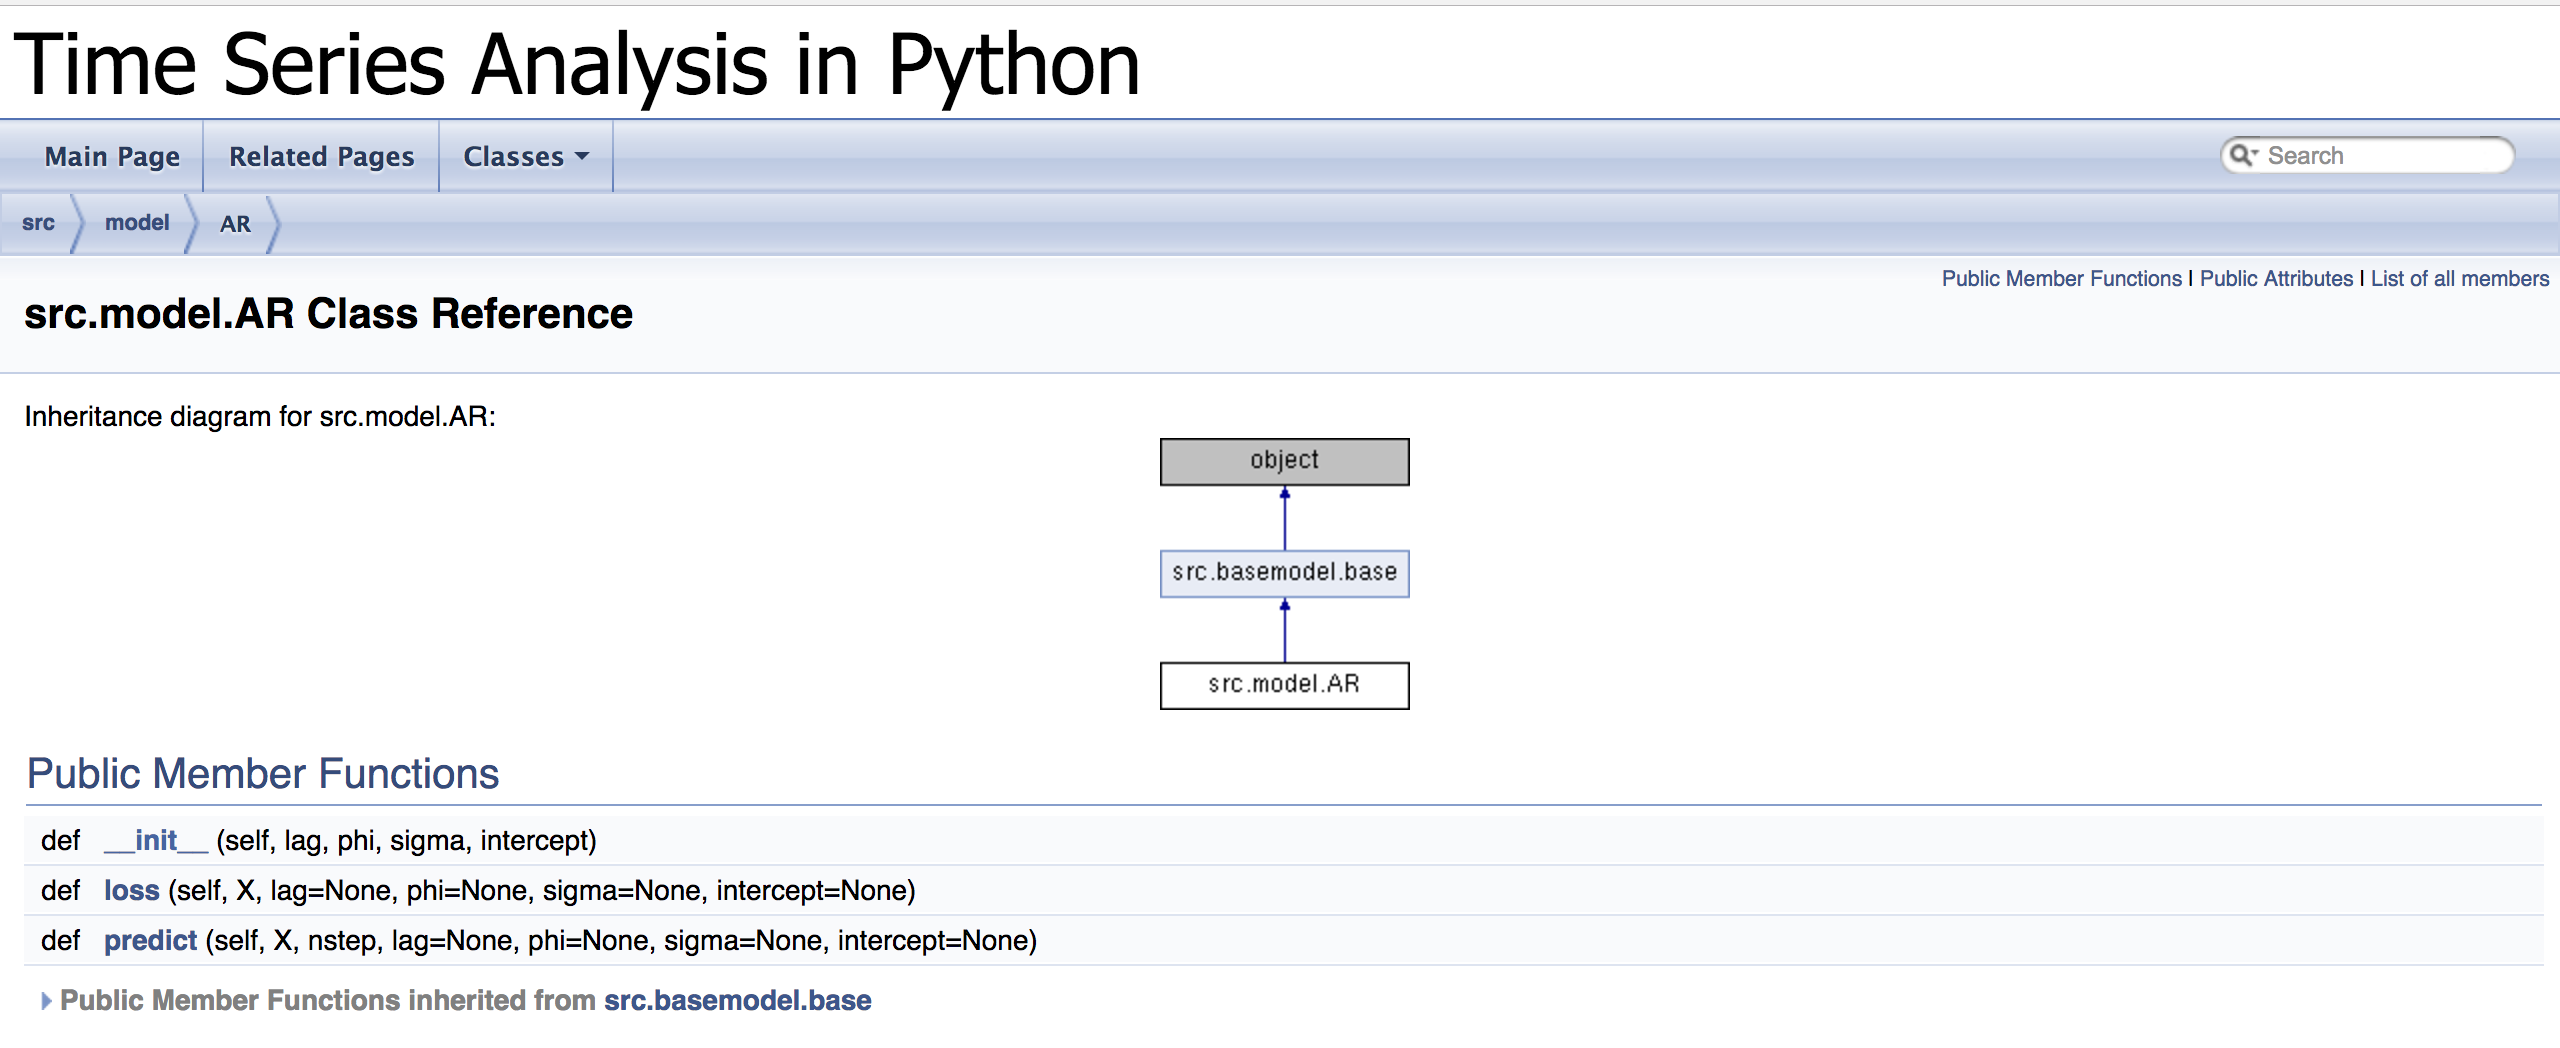
\includegraphics[width=.7\linewidth]{./Figure/Doxygen.png}
\caption{Doxygen documentation}
\end{figure}

We have a few milestones for this project. (1) Prototype, Dec 15. In this release, we had at least one implementation for each step. Then given a time series data, we could apply at least one method from each class to do the analysis. (2) Alpha version, Jan 1. In this release, we completed most methods in each class. (3) Final version, Jan 12.  In this relase, we finalized the project. Finish all the testing using various data including simulated data and real finanical data.

\section{Architecture}
The high-level program structure is shown below. The division of work is pretty even, and there are some minor work that are too trivial to mention extensively here. Overall, the program consists of two parts. The first part deal with a single time series, and exploits the time correlation within the time series. There is data preprocessing module that takes the raw data and get the right dataformat for later analysis. Optimization, model, and solver are used all together to identify the models. Finally, there is a post processing module that makes use of the information from model. The post processing module includes parameter inference, trading strategy, and option pricing. The second part deals with a collection of time series of data, basically it exploits the correlation between different time series. In this way, we can gain more insights into the finanical market. While these insights are impossible for a single time series.
\begin{figure}[H]
        \centering
     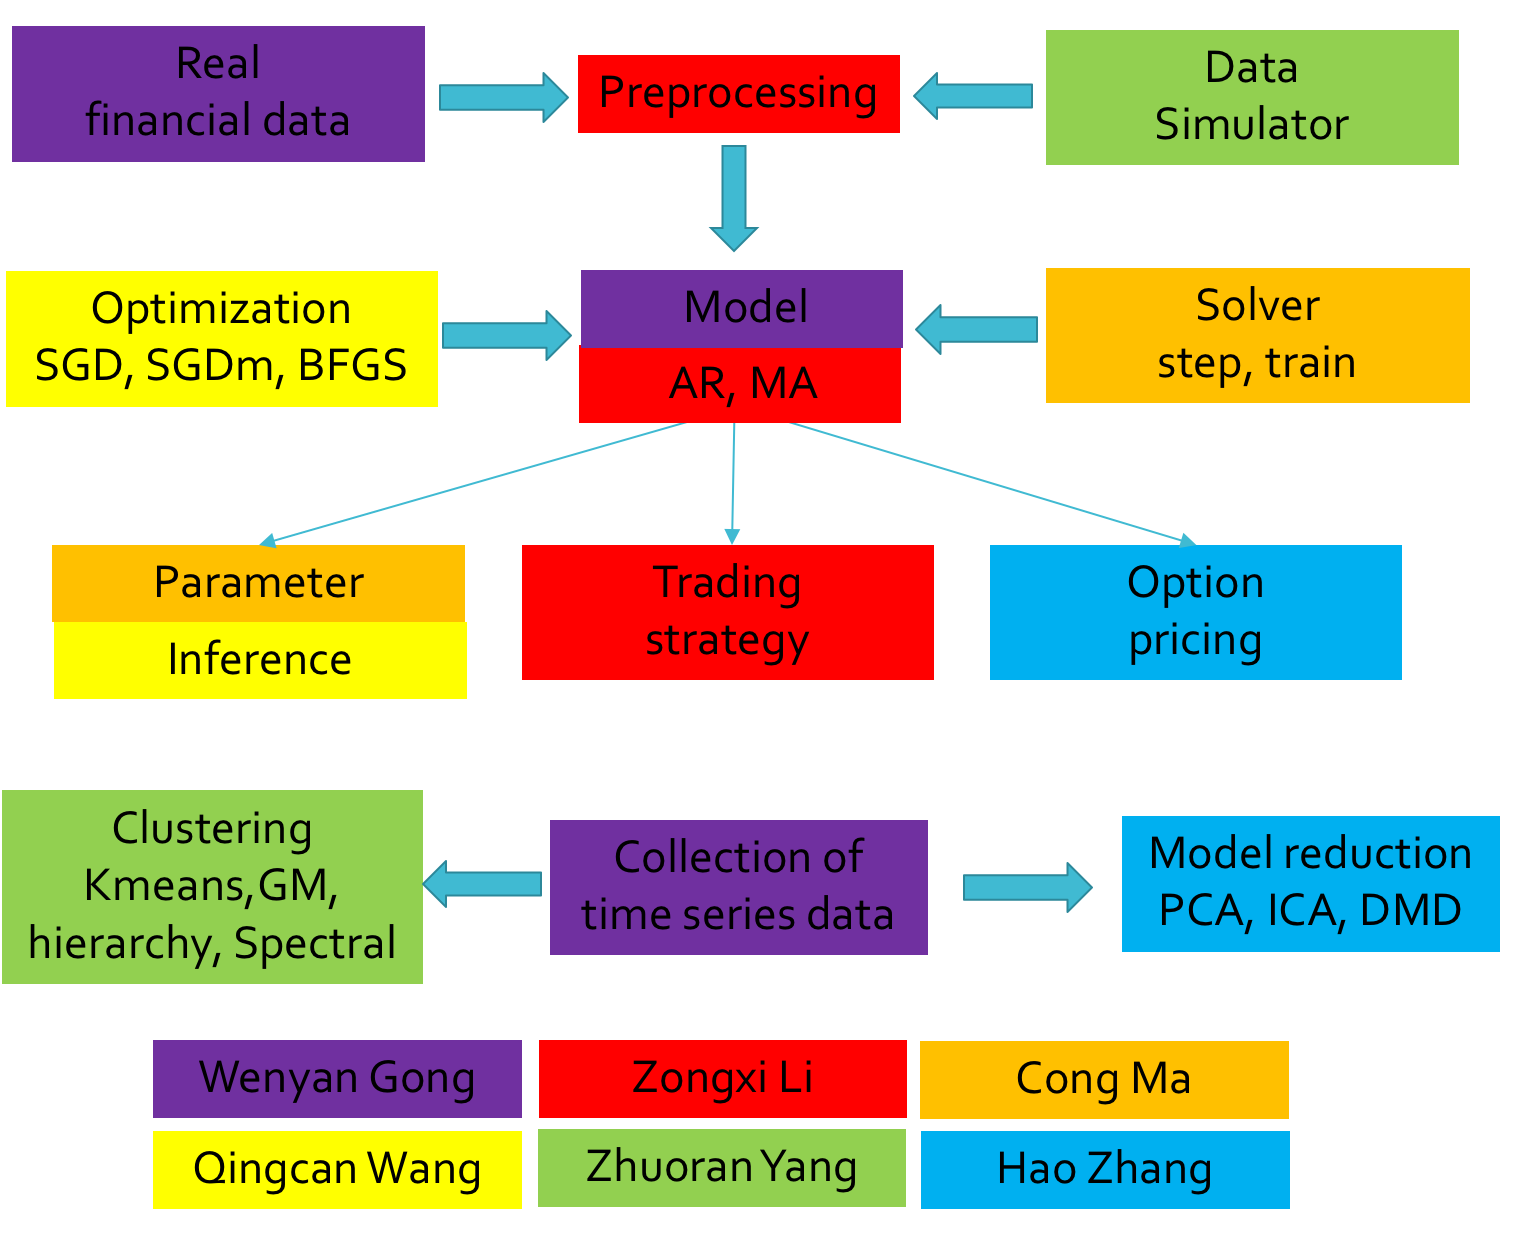
\includegraphics[width=.5\linewidth]{./Figure/structure.png}
\caption{Program structure and division of work}
\end{figure}

\subsection{Data collection \& preprocessing}
We develop simulator to simulate data for model testing. At the same time, real finanical data (S\&P 500) are also collected from online source.

\subsection{Model}
For a given time series, there are several potential classes of models that could be used to describe its variation. Among them, the most frequent used are the autoregressive(AR) model, integrated(I) model and the moving-average(MA) model. The combination of these classes lead to the autoregres- sive moving-average(ARMA) model, the autoregressive integrated moving-average(ARIMA) model and the autoregressive fractionally integrated moving-average(ARFIMA) model. The user could choose the model class he/she wish to fit based on his understanding of the input time series.

\subsection{Optimization}
%!TEX root = ../../manual.tex

The optimization part \texttt{optim.py} implements various optimization update
rules: stochastic gradient descent (\texttt{sgd}), stochastic gradient descent
with momentum update (\texttt{sgd\_momentum}) and
Broyden–Fletcher–Goldfarb–Shanno algorithm (\texttt{bfgs}). 

Each update rule accepts current iteration point and the gradient of the object
function and produces the next iteration point. Each update rule has the same
interface:
\begin{lstlisting}[language=Python]
def update(x, dx, config=None):
\end{lstlisting}
The inputs are as follows:
\begin{enumerate}
  \item \texttt{x}:
    A \texttt{numpy} array giving the current iteration point.
  \item \texttt{dx}:
    A \texttt{numpy} array of the same shape as \texttt{x} giving the gradient
    of the object function with respect to \texttt{x}.
  \item \texttt{config}:
    A dictionary containing hyper-parameter values such as learning rate,
    momentum, etc. If the update rule requires caching values over many
    iterations, then config will also hold these cached values.
\end{enumerate}
The outputs are as follows:
\begin{enumerate}
  \item \texttt{next\_x}:
    The next point after the update.
  \item \texttt{config}:
    The config dictionary to be passed to the next iteration of the update rule.
\end{enumerate}

The update rules are called in \texttt{Solver} class like this:
\begin{lstlisting}[language=Python]
objfcn, grads = self.model.objfcn(self.X)
for p, x in self.model.params.iteritems():
    dx = grads[p]
    config = self.optim_configs[p]
    next_x, next_config = self.update_rule(x, dx, config)
    self.model.params[p] = next_x
    self.optim_configs[p] = next_config
\end{lstlisting}




\subsection{Solver}
%!TEX root = ../../report.tex
We develop a solver class, which serves as a bridge between the model class and the optimization methods. Specifically, given the loss function and the gradient functions specified by the model and the optimization methods, the solver uses this method to minimize the loss until it converges. 

\subsection{Inference}
After model fitting, in order to provide the user with more overall information about the model, our software also do inference work regarding the parameters. The software would construct confidence interval of given level for each parameter, conduct test to decide the non-zero parameters and calculate the corresponding P-value. This could help to identify the pattern of the model and help the user develop deeper understanding of the given time series.

\subsection{Trading strategy}
The software is able to predict the future price for each stock based on the fitted model. Hence, in the data visualization part, it would plot the estimated future price and an prediction interval along with the previous price that is already known. Together, some trading strategy would be made based on the prediction. The software could provide the user with the selling or buying point of certain stocks.

\subsection{Option pricing}
%!TEX root = ../../manual.tex

The class \texttt{OptionPricing} calculates the call option price of an underlying
stock based on the Black-Scholes model.

The following parameters are needed to construct an instance of the
\texttt{OptionPricing} class:
\begin{enumerate}
  \item \texttt{sigma}:
    the volatility of the underlying stock price, which is the standard
    deviation of the stock's returns.
  \item \texttt{K}:
    the strike price of the option.
  \item \texttt{T}:
    the expiry time of the option.
  \item \texttt{r}:
    the risk-free interest rate.
  \item \texttt{Smax}:
    the maximum stock price we want to consider.
\end{enumerate}

The method \texttt{solve\_black\_scholes} calculates the option pricing of an
instance, given the grid size of price and time (\texttt{nS} and \texttt{nt}) as
input parameters. The option price as an function of stock price and time will
be stored in the instance.

After running \texttt{solve\_black\_scholes}, we can use 
\texttt{get\_option\_price} method to get the option price of given underlying
stock price \texttt{S} and time \texttt{t}.

Following is a usage example of the \texttt{OptionPricing} class:
\begin{lstlisting}[language=Python]
goog = np.genfromtxt("../data/GOOG.csv", delimiter=",")
sigma = np.std((goog[1:] - goog[:-1]) / goog[:-1])

option_price = OptionPricing(sigma=sigma, T=90, K=800, r=0.005, Smax=1200)
option_price.solve_black_scholes(nS=100, nt=300)
print(option_price.get_option_price(S=810, t=30))
\end{lstlisting}



%!TEX root = ../../report.tex

\subsection{Clustering}
In order to handle the cope with heterogeneous datasets, i.e., datasets with various  characteristics, we provide clustering methods that enable users to perform data analysis with more accuracy.  By utilizing clustering tools, users may discover hidden structures shared by a small subgroup of the dataset  that are buried due to the large scale of the hole dataset. 

To better understand the importance of clustering, let us consider the example of stock market, which consists of stocks that  belong to various sectors. Although there is a global trend of the market as a whole, various sectors may exhibit  different, even converse movements. Thus, global information can be too crude to perform more fine-grained analysis; it would cause huge error if the user predicts the trend of energy stocks using data coming from the whole market.

In the package, we provide a variety of commonly used clustering methods, which include k-means, hierarchical clustering,  spectral clustering, and Gaussian mixture modeling. See   \cite{elsbook} and \cite{bishop2006pattern} for introduction of clustering methods. Our methods yield results  comparable with other machine learning packages in \texttt{python}. In specific, in \texttt{demo\_clustering.ipynb} we showcase our method and  compare with the \texttt{Scikit-Learn} package using the \texttt{S\&P 500} dataset, which consists of the prices of $470$ stocks in a period of $490$ days. A concise illustration is provided in the next section.

\subsection{Model reduction}
model reduction

program structure, division of work, user interface, 
independent component analysis \cite{hyvarinen2000independent}.

\section{Demos of results}
\subsection{Modal validation}
\subsection{Finanical data}
\subsection{Trading strategy}
\subsection{Option pricing}
\subsection{Clustering}
\subsection{Model reduction}

\section{Lessons learned}

\bibliography{ref}
\end{document}